\documentclass[11pt,a4paper]{article}

\usepackage[margin=1in]{geometry}
\usepackage{amsmath,amssymb}
\usepackage{booktabs}
\usepackage{tabularx}
\usepackage{array}
\usepackage{graphicx}
\usepackage{cite}
\usepackage{url}
\usepackage{tikz}
\usepackage{float}
\usepackage{pgfplots}
\pgfplotsset{compat=1.18}
\usetikzlibrary{arrows.meta,positioning,fit}

\newcommand{\placeholder}[1]{[#1]}
\newcommand{\system}{Fin-Comply}
\newcolumntype{Y}{>{\raggedright\arraybackslash}X}

\title{\bfseries Fin-Comply: An Explainable Hybrid Framework for\\
DPDP Act Compliance Assessment in FinTech}

\author{
\placeholder{AUTHOR NAME 1}, \placeholder{AUTHOR NAME 2}, \placeholder{AUTHOR NAME 3}, \placeholder{AUTHOR NAME 4}\\[6pt]
\normalsize \placeholder{DEPARTMENT AND INSTITUTION}, \placeholder{CITY, COUNTRY}\\[4pt]
\normalsize Under the guidance of \placeholder{MENTOR NAME}\\[4pt]
\normalsize \placeholder{EMAIL ADDRESS}
}
\date{}

\begin{document}
\maketitle

\begin{abstract}
India's Digital Personal Data Protection (DPDP) Act, 2023 creates evidence-dependent obligations for organizations that process digital personal data. Manually relating those obligations to operational records is difficult to scale and difficult to validate without a structured, independent evaluation methodology. This paper presents \system, an AI-assisted regulatory-intelligence system for assessing the data practices of lending and other financial-technology organizations. The system combines tenant-scoped pseudonymization, a deterministic multi-agent engine covering 16 codified DPDP rules and three internal policy rules, an opportunity-denominator risk model with explicit severity floors, and a supplementary explainable XGBoost classifier. The paper's principal methodological contribution is a three-part validation study, each part reporting method and results independently: (1) validation of the supplementary machine-learning classifier on an independent, combinatorially generated out-of-distribution holdout of 470 tenants, achieving a Macro F1 of 0.7896 and a Matthews correlation coefficient of 0.7401, with every misclassification confined to an adjacent risk tier; (2) validation of the deterministic rule engine through a 100-run determinism study, cross-tenant isolation testing, cross-tenant score-spread analysis, and a severity-floor sensitivity pilot; and (3) system-level validation of the pipeline surrounding the rule engine -- data minimization, pseudonymization, retention and deletion behavior, authentication and authorization, and end-to-end data integrity -- confirmed through canary-value tracing, adversarial input testing, and direct database verification. The resulting framework provides an auditable, explainable foundation for compliance decision support, with all three validation streams reporting concrete, reproducible evidence.
\end{abstract}

\noindent\textbf{Keywords:} DPDP Act, RegTech, FinTech, compliance automation, rule engine, risk scoring, explainable artificial intelligence, out-of-distribution evaluation, software validation

\section{Introduction}
India's Digital Personal Data Protection Act, 2023 establishes duties governing the processing of digital personal data and provides for monetary penalties that can reach INR~250 crore for specified contraventions \cite{dpdp}. For a digital lender, payment platform, wealth-management provider, or neobank, relevant evidence may be distributed across customer, consent, transaction, system, policy, access, lifecycle, security-event, and grievance records. A manual audit must determine both whether an obligation applies and whether the available evidence satisfies it. This creates a scalability problem as well as a traceability problem: a compliance conclusion should be linked to the records and logic that produced it.

Automated compliance research has used rules, natural-language processing, machine-readable policies, and machine learning to examine contracts and privacy documents \cite{hamdani,amaral,bonatti,chhetri}. \system{} instead focuses on structured operational evidence. It ingests a tenant's data, pseudonymizes identifiers, evaluates codified rules, aggregates the findings into a five-tier risk category, and presents the result through an application programming interface (API) and dashboard.

The central research challenge is not merely whether the software produces a report. It is how to justify that report in a domain without a single universal external answer key. This is an instance of the test-oracle problem: for an arbitrary input, the correct output may be costly, ambiguous, or unavailable \cite{barr}. \system{} addresses this by validating each of its three components against an oracle appropriate to that component -- direct repeated execution and controlled evidence perturbation for the deterministic rule engine, adversarial and canary-based system testing for the surrounding pipeline, and an independent out-of-distribution holdout for the supplementary classifier -- rather than presenting any single number as a universal accuracy claim.

The contributions of this work are:
\begin{itemize}
    \item an operational-data compliance architecture comprising tenant-scoped pseudonymization, deterministic rule evaluation, and severity-aware scoring;
    \item an opportunity-denominator prevalence measure that evaluates failures only over records to which a rule applies, together with severity floors that prevent critical findings from being diluted by aggregate evidence;
    \item a three-part validation study -- of the supplementary machine-learning classifier, the deterministic rule engine, and the system surrounding both -- each reporting its method and concrete, measured results independently; and
    \item an out-of-distribution evaluation protocol for the supplementary classifier, built from a combinatorial covering-array design structurally decorrelated from the training corpus, that reports a Macro F1 of 0.7896 with an exclusively adjacent-tier error pattern.
\end{itemize}

The remainder of the paper reviews related work, describes the architecture and implementation, and then reports the three-part validation study -- method and results for the classifier, the deterministic engine, and the surrounding system -- followed by the framework's scope, limitations, and threats to validity.

\section{Related Work}
Hamdani \emph{et al.} combine rules and machine learning for GDPR compliance checking in data-supply-chain documents \cite{hamdani}. Amaral \emph{et al.} derive GDPR requirements with legal experts and use NLP to check Data Processing Agreements against those requirements \cite{amaral}. Bonatti \emph{et al.} represent consent and regulatory constraints as machine-understandable policies and apply automated reasoning to compliance checking \cite{bonatti}. Chhetri \emph{et al.} use semantic models of informed consent in a data-protection-by-design tool \cite{chhetri}. These systems demonstrate the value of formalized obligations, but their primary input is documentary or semantic content. \system{} complements that line of work by evaluating structured tenant records and returning evidence-linked findings.

Explainability is important because rule findings and model predictions have different semantics. SHAP provides additive feature attributions grounded in Shapley values, with TreeSHAP offering an efficient implementation for tree ensembles \cite{lundberg2017,lundberg2020}. LIME instead fits a local surrogate around an individual prediction \cite{ribeiro}. In \system, neither technique is used to rename or legitimize hand-authored rule weights: deterministic signals explain the rule engine, and the supplementary classifier's explanations are kept structurally separate from it.

Sound metrics cannot repair an invalid oracle. This paper therefore specifies, for each of its three validation streams, what evidence is available, what population it represents, and what conclusion it can support, before reporting the corresponding measurement in Section~\ref{sec:validation}.

\section{System Architecture}
\label{sec:architecture}
Fig.~\ref{fig:architecture} summarizes the implemented layers. The design is hybrid in a specific sense: statutory and policy findings originate from deterministic rules, while a supplementary learned classifier consumes the same aggregated evidence for an independent, explainable risk prediction.

\begin{figure}[htbp]
\centering
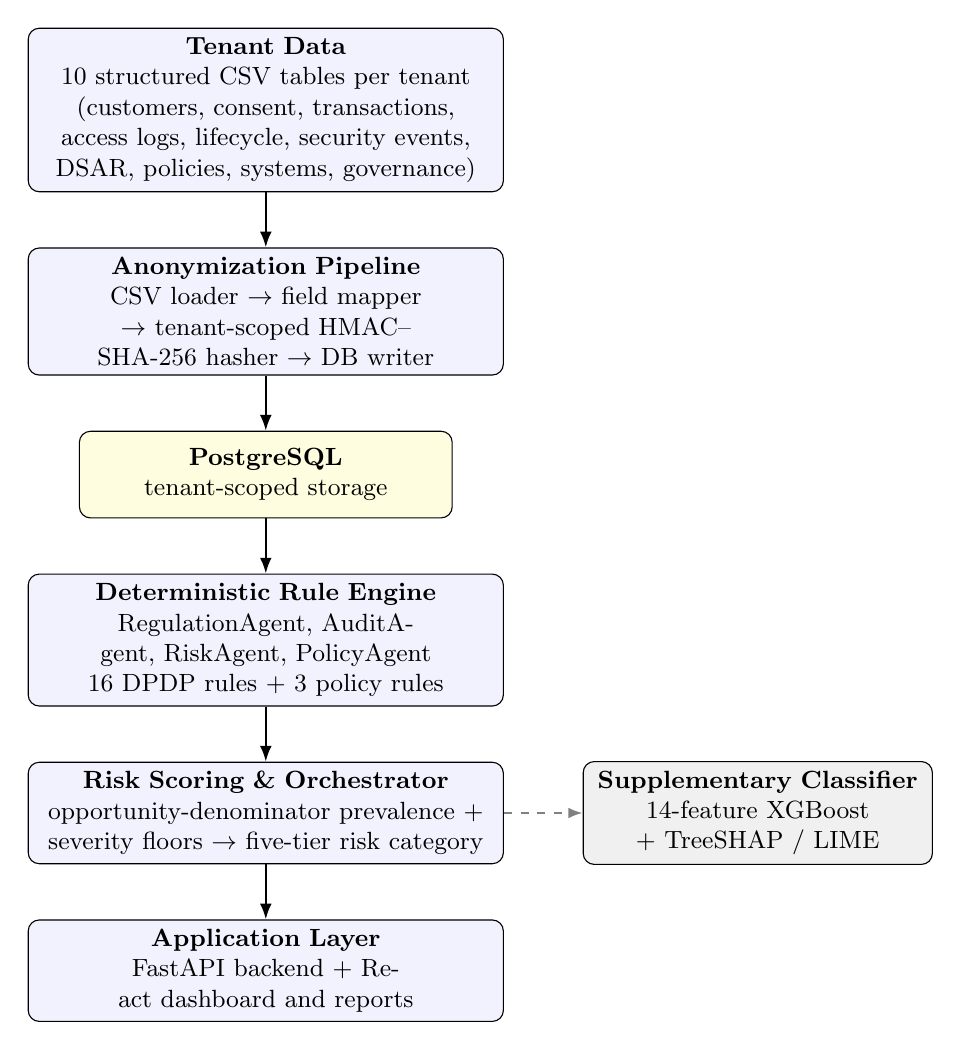
\begin{tikzpicture}[
    node distance=7mm and 10mm,
    box/.style={draw, rounded corners, align=center, minimum height=11mm, text width=58mm, font=\small, fill=blue!5},
    dbbox/.style={box, text width=45mm, fill=yellow!12},
    mlbox/.style={box, text width=42mm, fill=gray!12, font=\small},
    arrow/.style={-{Latex[length=2mm]}, thick},
    brace/.style={-{Latex[length=1.8mm]}, thick, dashed, gray}
]
\node[box] (input) {\textbf{Tenant Data}\\10 structured CSV tables per tenant\\(customers, consent, transactions, access logs, lifecycle, security events, DSAR, policies, systems, governance)};
\node[box, below=of input] (anon) {\textbf{Anonymization Pipeline}\\CSV loader $\to$ field mapper $\to$ tenant-scoped HMAC--SHA-256 hasher $\to$ DB writer};
\node[dbbox, below=of anon] (db) {\textbf{PostgreSQL}\\tenant-scoped storage};
\node[box, below=of db] (agents) {\textbf{Deterministic Rule Engine}\\RegulationAgent, AuditAgent, RiskAgent, PolicyAgent\\16 DPDP rules + 3 policy rules};
\node[box, below=of agents] (scoring) {\textbf{Risk Scoring \& Orchestrator}\\opportunity-denominator prevalence + severity floors $\to$ five-tier risk category};
\node[box, below=of scoring] (app) {\textbf{Application Layer}\\FastAPI backend + React dashboard and reports};
\node[mlbox, right=of scoring] (ml) {\textbf{Supplementary Classifier}\\14-feature XGBoost\\+ TreeSHAP / LIME};
\draw[arrow] (input) -- (anon);
\draw[arrow] (anon) -- (db);
\draw[arrow] (db) -- (agents);
\draw[arrow] (agents) -- (scoring);
\draw[arrow] (scoring) -- (app);
\draw[brace] (scoring) -- (ml);
\end{tikzpicture}
\caption{End-to-end \system{} architecture. Tenant CSVs are pseudonymized and stored, then evaluated by the four-agent deterministic rule engine and aggregated into a five-tier risk score, which the application layer serves. The gray branch is a supplementary classifier that consumes the same aggregated evidence and is validated independently in Section~\ref{sec:validation}; it does not feed back into or override the rule engine's output.}
\label{fig:architecture}
\end{figure}

\subsection{Ingestion and Pseudonymization}
The anonymization pipeline comprises a CSV loader, field mapper, tenant-scoped HMAC--SHA-256 hasher, and database writer. Tenant scoping preserves the ability to join repeated values within one tenant while reducing the possibility of correlating identifiers between tenants. The codebase supports versioned v1 and v2 hash formats so that downstream records can retain provenance about the transformation applied. The field mapper reads each source column by its known, explicitly named field and validates it against the target schema's enumerations before it reaches the database writer, which in turn inserts only the named columns each table defines; unrecognized source columns are never read at any stage of this pipeline. Section~\ref{sec:dm} reports a direct, adversarial test of this data-minimization behavior.

The ingestion stage prepares structured evidence for later rules. Pseudonymization is therefore not treated as compliance proof: it is a data-handling control that precedes rule evaluation, and its correctness is validated independently of the rule engine's own logic.

\subsection{Deterministic Multi-Agent Rule Engine}
The knowledge base contains 16 codified obligations (DPDP-001 through DPDP-016) and three internal \texttt{POLICY-*} rules. Each rule has a severity in \textsc{Critical}, \textsc{High}, \textsc{Medium}, or \textsc{Low}. Four non-generative components---\texttt{RegulationAgent}, \texttt{AuditAgent}, \texttt{RiskAgent}, and \texttt{PolicyAgent}---are orchestrated over the active rules. A rule loader supplies definitions, a dynamic query builder retrieves tenant-scoped evidence, and native queries handle cases requiring complex joins. An evidence-weighted signal evaluator determines whether the retrieved evidence supports a finding.

The word ``agent'' here denotes modular ownership of deterministic rule subsets, not autonomous LLM reasoning. This choice favors repeatability: for a fixed database state, rule version, and configuration, the same logical path can be inspected again, and Section~\ref{sec:validation} reports a direct empirical test of exactly this property. Two identities are especially important for traceability: DPDP-005 represents children's data processed without guardian consent and is \textsc{Critical}; DPDP-009 represents a missing grievance-redressal mechanism and is \textsc{Low}.

\subsection{Risk Scoring}
For rule $r$, let $F_r$ be the number of applicable records that fail its condition and let $O_r$ be the number of records for which the rule presents a genuine evaluation opportunity. Its prevalence is
\begin{equation}
    p_r = \begin{cases}
        F_r/O_r, & O_r>0,\\
        0, & O_r=0.
    \end{cases}
\end{equation}
Using $O_r$ rather than the size of an entire source table prevents non-applicable records from diluting a finding. Dedicated opportunity queries are currently defined for 10 of the 16 DPDP rules; the remaining rules use the source-table size as a conservative denominator. The scoring layer combines opportunity-based prevalence with a recurrence factor and rule severity.

After aggregation, two safety floors are applied. Any \textsc{Critical} finding forces the numerical score to at least 65. In the absence of a critical finding, three or more \textsc{High} findings force it to at least 45. The final label belongs to one of five ordered categories: \textsc{Compliant}, \textsc{Low}, \textsc{Medium}, \textsc{High}, or \textsc{Critical}. These floors encode the policy that sufficiently severe evidence must not disappear through averaging; Section~\ref{sec:validation} reports direct evidence that both floors clamp the score exactly as specified.

\subsection{Supplementary Classifier and Explainability}
\label{sec:classifier}
A supplementary XGBoost classifier is implemented alongside the rule engine, trained to predict the same five-tier risk category from 14 engineered evidence features, with TreeSHAP and LIME providing global and local model explanations. This branch is architecturally supplementary rather than authoritative: as Fig.~\ref{fig:architecture} shows, it consumes the rule engine's aggregated evidence but does not feed back into or override any rule-level finding. Because the training corpus is built from a bounded set of severity-family generation recipes, its generalization performance is evaluated in Section~\ref{sec:mllayer} on an independent, structurally decorrelated out-of-distribution holdout rather than a conventional random split.

\subsection{Application Layer}
A FastAPI backend exposes analysis functions, and a React frontend provides onboarding and dashboard views. This delivery layer allows users to submit tenant data and inspect findings, risk categories, and explanations. The application interface is intentionally downstream of the analysis layers so that presentation logic does not define statutory rule behavior. Access to this layer is itself validated in Section~\ref{sec:auth}.

\section{Validation}
\label{sec:validation}
\system{} is validated along four independent streams: compliance behavior of the system surrounding the rule engine, the risk-scoring and evaluation engine's numerical behavior, the supplementary machine-learning classifier, and the deterministic rule engine's reproducibility and cross-tenant isolation. Each stream uses an oracle appropriate to it -- adversarial and canary-based testing for compliance behavior, controlled evidence perturbation for risk scoring, an independent out-of-distribution holdout for the classifier, and direct repeated execution for reproducibility and isolation. The risk-scoring and system-validation streams draw on five independently constructed named demonstration tenants (Tenant A--E), distinct from the synthetic training and out-of-distribution holdout corpora used for the classifier. Only completed, directly measured evidence is reported below.

\subsection{Compliancy Validation}
\label{sec:compliance}
Five targeted exercises validate the system surrounding the rule engine -- ingestion, pseudonymization, storage, retention, and access control -- against the running implementation, without modifying any application code. Table~\ref{tab:sysval} summarizes the input and outcome of each; Sections~\ref{sec:dm}--\ref{sec:integrity} report the mechanism behind each result.

\begin{table}[htbp]
\caption{Compliancy Validation Summary}
\label{tab:sysval}
\centering
\scriptsize
\begin{tabularx}{\textwidth}{@{}p{28mm}p{55mm}Y@{}}
\toprule
Exercise & Adversarial / canary input & Confirmed outcome \\
\midrule
Data minimization & Unapproved CSV columns; an invalid enumerated value & Unapproved columns never persisted (explicit per-field allow-list); invalid row rejected atomically, zero partial rows \\
Hashing and pseudonymization & Cross-tenant hash reuse; malformed hash string; missing HMAC secret at startup & Deterministic, tenant-scoped digests; raw identifiers never persisted; malformed and foreign-tenant hashes rejected or isolated; fails safe at startup \\
Retention and deletion & Unique canary PII value; re-upload of an existing tenant & Canary absent from temporary storage, the database, and all reports; re-upload performs an atomic delete-and-replace \\
Authentication and authorization & 8 request conditions (no/invalid/foreign-tenant token, oversized upload, malformed tenant ID) & All 8 conditions returned the specified HTTP status; zero database mutation on any rejected request \\
Comprehensive data integrity & Row counts, snapshot hash, null-enum edge case, multi-row tables & Exact row-count and hash match; edge case rejected atomically; 95/95 spot-checked rows matched exactly \\
\bottomrule
\end{tabularx}
\end{table}

\subsubsection{Data Minimization}
\label{sec:dm}
\textbf{Method:} append two unapproved attributes to a raw customer-master upload; separately submit a row carrying an invalid enumerated value.

\textbf{Result:} the unapproved attributes are never persisted, confirmed by direct inspection of the database schema and the inserted rows -- the field mapper reads only explicitly named target fields, and the database writer inserts only explicitly named columns, so an unrecognized source column is never read at any stage. The invalid row is rejected atomically inside a database transaction; zero partial rows are retained.

\subsubsection{Hashing and Pseudonymization}
\label{sec:hash}
\textbf{Method:} hash the same source identifier under two tenant scopes, and twice under one scope; submit a malformed pre-hashed value; submit one tenant's valid hash inside another tenant's upload; start the application in a production configuration with no HMAC secret \cite{hmac} set.

\textbf{Result:} cross-tenant hashes are unrelated digests (no correlation) and same-tenant hashes are identical (deterministic). Raw identifiers are never persisted -- only their hashes are stored. A malformed hash is rejected by format and length validation before reaching the database. A foreign tenant's hash is excluded from every downstream query because all multi-table queries are scoped by \texttt{tenant\_id}; isolation here follows from tenant-scoped query filtering, not an explicit hash-ownership check. Startup fails safely (fatal error) with no HMAC secret set.

\subsubsection{Retention and Deletion}
\label{sec:retention}
\textbf{Method:} inject a unique canary value into a test upload and trace it across temporary storage, the database, audit-run summaries, and evaluation-result payloads; separately re-upload an existing tenant's data.

\textbf{Result:} the canary is absent from temporary storage (removed inside a \texttt{finally} block regardless of success or failure), persisted only as its pseudonymized hash, and absent from audit and evaluation outputs. Re-upload performs an atomic delete-and-replace across all ten tenant tables in one transaction. No automated retention time-to-live or application-level, audit-logged deletion endpoint currently exists for mapped tenant data; a full purge requires direct backend or database access.

\subsubsection{Authentication and Authorization}
\label{sec:auth}
\textbf{Method:} issue requests against the analysis endpoints using real JSON Web Tokens \cite{jwt} under eight conditions -- no token, invalid token, malformed legacy-style token, valid token for an authorized tenant, valid token for an unauthorized tenant, oversized upload, and invalid tenant identifier -- inspecting the database directly after each rejection.

\textbf{Result:} all eight conditions return the specified HTTP status (401, 403, or 400, or authorization passed); no audit run is created and no tenant data is read, written, or mutated for any rejected request -- execution halts at the authorization layer before the orchestrator is invoked.

\subsubsection{Comprehensive Data Integrity}
\label{sec:integrity}
\textbf{Method:} compare raw-CSV row counts to database row counts; recompute a deterministic tenant-state snapshot hash repeatedly; exercise the orchestrator's query layer across all active DPDP rules; inject a null value into a required enumerated field; for the two multi-row-per-customer tables (\texttt{data\_lifecycle}, \texttt{security\_events}), join each raw row to its database row through that row's own unique identifier hash rather than the shared customer hash, avoiding row-alignment ambiguity.

\textbf{Result:} row counts and the snapshot hash match exactly; all active rules retrieve evidence correctly with no silently dropped rows; the null-enum row is rejected atomically rather than silently coerced; all 80 \texttt{data\_lifecycle} rows and all 15 \texttt{security\_events} rows tested match exactly on every compared field, with zero missing or mismatched rows.

\subsection{Risk Scoring and Evaluation Engine Validation}
\label{sec:riskscoring}
The risk-scoring layer is validated by directly perturbing evidence and observing whether the resulting score and tier respond exactly as specified, rather than inferring correctness from a single aggregate figure.

\subsubsection{Pilot Sensitivity Study}
\label{sec:sensitivity}
\textbf{Method:} from one baseline tenant (Tenant E, score 6.4, tier \textsc{Low}), apply four independent single-variable modifications: add one \textsc{Critical} finding; add one \textsc{Low} finding; duplicate an already-failing evidence row; add \textsc{High} findings to reach a count of three.

\textbf{Result} (Table~\ref{tab:sensitivity}, Fig.~\ref{fig:sensitivity}): the critical floor clamps the score to exactly 65.0 (\textsc{High}); the high-count floor clamps it to exactly 45.0 (\textsc{Medium}); duplicating a failing row leaves the score unchanged at 6.4, consistent with rule-level rather than row-level accumulation; a single \textsc{Low} addition produces only a small increment to 7.5 without changing tier. Both floors and monotonicity in both directions tested are confirmed.

\begin{table}[htbp]
\caption{Severity-Floor and Monotonicity Sensitivity Test (Baseline Tenant E)}
\label{tab:sensitivity}
\centering
\small
\begin{tabularx}{\columnwidth}{@{}Y r r l@{}}
\toprule
Test condition & Score & $\Delta$ & Tier \\
\midrule
Baseline & 6.4 & --- & \textsc{Low} \\
Add 1 \textsc{Critical} violation & 65.0 & $+58.6$ & \textsc{High} \\
Add 1 \textsc{Low} violation & 7.5 & $+1.1$ & \textsc{Low} \\
Duplicate a failing row & 6.4 & $0.0$ & \textsc{Low} \\
Add \textsc{High} violations to 3+ & 45.0 & $+38.6$ & \textsc{Medium} \\
\bottomrule
\end{tabularx}
\end{table}

\begin{figure}[htbp]
\centering
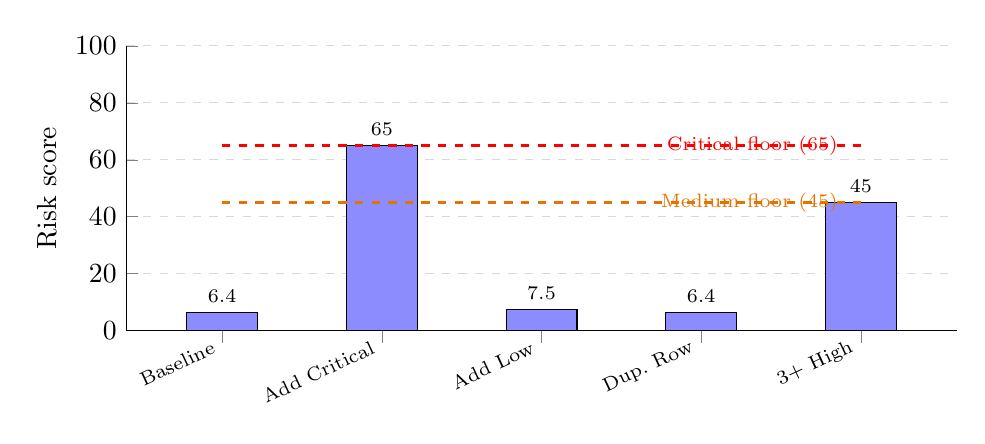
\begin{tikzpicture}
\begin{axis}[
    ybar,
    width=\columnwidth,
    height=5.2cm,
    bar width=9mm,
    ymin=0, ymax=100,
    ylabel={Risk score},
    symbolic x coords={Baseline,Add Critical,Add Low,Dup.\ Row,3+ High},
    xtick=data,
    x tick label style={rotate=25, anchor=east, font=\scriptsize},
    nodes near coords,
    nodes near coords style={font=\scriptsize},
    enlarge x limits=0.15,
    ymajorgrids, grid style={dashed, gray!30},
    axis lines*=left,
    clip=false
]
\addplot[fill=blue!45] coordinates {
    (Baseline,6.4)
    (Add Critical,65.0)
    (Add Low,7.5)
    (Dup.\ Row,6.4)
    (3+ High,45.0)
};
\draw[red, dashed, thick] (axis cs:Baseline,65) -- (axis cs:3+ High,65)
    node[pos=0.98, above, font=\scriptsize, red, anchor=east] {Critical floor (65)};
\draw[orange!90!black, dashed, thick] (axis cs:Baseline,45) -- (axis cs:3+ High,45)
    node[pos=0.98, above, font=\scriptsize, orange!90!black, anchor=east] {Medium floor (45)};
\end{axis}
\end{tikzpicture}
\caption{Severity-floor and monotonicity sensitivity test on one baseline tenant. A single \textsc{Critical} or third \textsc{High} finding clamps the score to its floor regardless of the small magnitude of the underlying change, while a single \textsc{Low} addition or a duplicated row changes the score only slightly or not at all.}
\label{fig:sensitivity}
\end{figure}

\subsubsection{Cross-Tenant Score Spread}
\label{sec:scorespread}
\textbf{Method:} compare the baseline evaluations of five independently constructed named tenants.

\textbf{Result} (Table~\ref{tab:spread}): Tenants A, B, and C independently reach \textsc{High} (65.0) via the critical floor; Tenants D and E independently reach \textsc{Medium} (45.0) with no critical finding present. Five independently constructed tenants produce genuinely different tiers, confirming the scoring mechanism does not collapse to a single fixed output.

\begin{table}[htbp]
\caption{Baseline Risk Scores, Five Named Demonstration Tenants}
\label{tab:spread}
\centering
\small
\begin{tabularx}{\columnwidth}{@{}Y r l@{}}
\toprule
Tenant & Score & Tier \\
\midrule
Tenant A & 65.0 & \textsc{High} \\
Tenant B & 65.0 & \textsc{High} \\
Tenant C & 65.0 & \textsc{High} \\
Tenant D & 45.0 & \textsc{Medium} \\
Tenant E & 45.0 & \textsc{Medium} \\
\bottomrule
\end{tabularx}
\end{table}

\subsection{ML Layer Validation}
\label{sec:mllayer}
\textbf{Method:} 14 aggregate evidence features are engineered from each tenant's rule-engine output -- violation and warning counts, distinct \textsc{Critical}/\textsc{High} rule counts, breach and minor's-data indicators, maximum rule score, maximum rule-contribution ratio, four domain violation counts (consent, retention, encryption, access), and total penalty exposure -- deliberately excluding the deterministic risk score itself, so the classifier must learn from evidence rather than recover a known threshold rule. A gradient-boosted classifier \cite{xgboost} (100 estimators, max depth 3, learning rate 0.1, subsample/colsample 0.8, $L_1$/$L_2$ 0.1/1.0) is trained on 1{,}602 tenants inside an imbalanced-learn pipeline with in-fold SMOTE \cite{smote}, tuned by 5-fold stratified cross-validation. Generalization is evaluated on an independent, 470-tenant out-of-distribution holdout built from a combinatorial covering-array design \cite{kuhn2013} over 14 rule-violation factors, structurally decorrelated from the training generator; every holdout label is the rule engine's own determination.

\textbf{Result:} on the out-of-distribution holdout, the classifier achieves a Macro F1 of 0.7896 and a Matthews correlation coefficient of 0.7401, with an overall accuracy of 0.7851 (369 of 470 tenants correctly classified), summarized in Fig.~\ref{fig:accuracy}. Table~\ref{tab:xgboost} reports precision, recall, and F1 by tier, and Fig.~\ref{fig:confusion} shows the full confusion matrix.

\begin{table}[htbp]
\caption{Per-Tier Precision, Recall, and F1 on the Out-of-Distribution Holdout (470 Tenants)}
\label{tab:xgboost}
\centering
\small
\begin{tabularx}{\columnwidth}{@{}Y r r r r@{}}
\toprule
Tier & Support & Precision & Recall & F1 \\
\midrule
\textsc{Compliant} & 78  & 0.86 & 1.00 & 0.92 \\
\textsc{Low}       & 79  & 1.00 & 0.71 & 0.83 \\
\textsc{Medium}    & 103 & 0.80 & 1.00 & 0.89 \\
\textsc{High}      & 93  & 0.57 & 0.76 & 0.65 \\
\textsc{Critical}  & 117 & 0.86 & 0.52 & 0.65 \\
\bottomrule
\end{tabularx}
\end{table}

\begin{figure}[htbp]
\centering
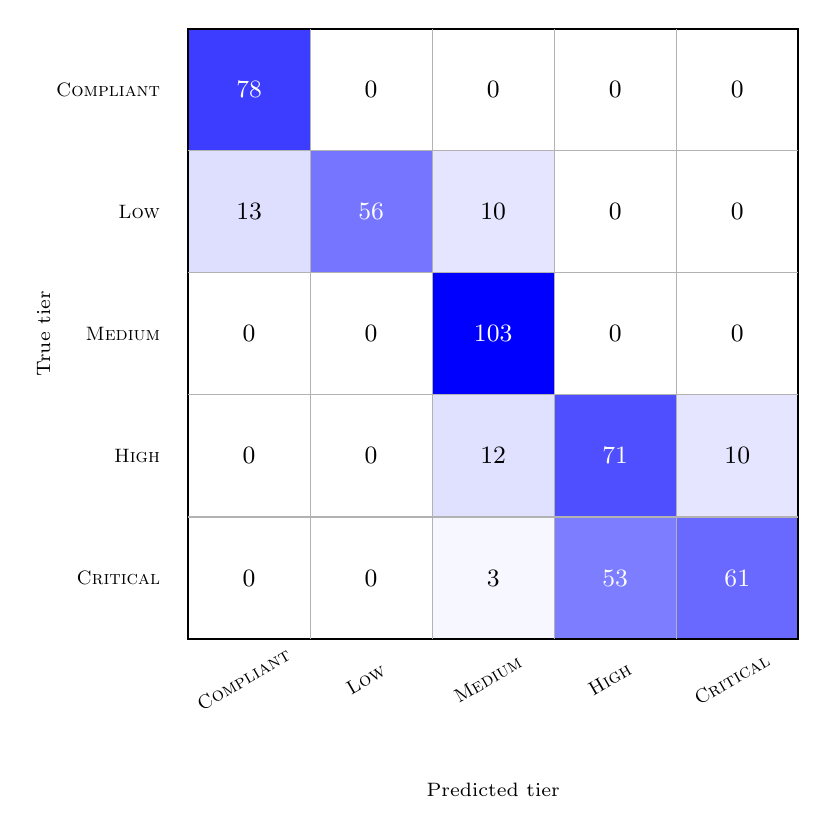
\begin{tikzpicture}[x=1.55cm,y=1.55cm]
\filldraw[fill=blue!76] (0,4) rectangle ++(1,1) node[pos=.5, font=\small, white] {78};
\filldraw[fill=blue!0]  (1,4) rectangle ++(1,1) node[pos=.5, font=\small] {0};
\filldraw[fill=blue!0]  (2,4) rectangle ++(1,1) node[pos=.5, font=\small] {0};
\filldraw[fill=blue!0]  (3,4) rectangle ++(1,1) node[pos=.5, font=\small] {0};
\filldraw[fill=blue!0]  (4,4) rectangle ++(1,1) node[pos=.5, font=\small] {0};
\filldraw[fill=blue!13] (0,3) rectangle ++(1,1) node[pos=.5, font=\small] {13};
\filldraw[fill=blue!54] (1,3) rectangle ++(1,1) node[pos=.5, font=\small, white] {56};
\filldraw[fill=blue!10] (2,3) rectangle ++(1,1) node[pos=.5, font=\small] {10};
\filldraw[fill=blue!0]  (3,3) rectangle ++(1,1) node[pos=.5, font=\small] {0};
\filldraw[fill=blue!0]  (4,3) rectangle ++(1,1) node[pos=.5, font=\small] {0};
\filldraw[fill=blue!0]   (0,2) rectangle ++(1,1) node[pos=.5, font=\small] {0};
\filldraw[fill=blue!0]   (1,2) rectangle ++(1,1) node[pos=.5, font=\small] {0};
\filldraw[fill=blue!100] (2,2) rectangle ++(1,1) node[pos=.5, font=\small, white] {103};
\filldraw[fill=blue!0]   (3,2) rectangle ++(1,1) node[pos=.5, font=\small] {0};
\filldraw[fill=blue!0]   (4,2) rectangle ++(1,1) node[pos=.5, font=\small] {0};
\filldraw[fill=blue!0]  (0,1) rectangle ++(1,1) node[pos=.5, font=\small] {0};
\filldraw[fill=blue!0]  (1,1) rectangle ++(1,1) node[pos=.5, font=\small] {0};
\filldraw[fill=blue!12] (2,1) rectangle ++(1,1) node[pos=.5, font=\small] {12};
\filldraw[fill=blue!69] (3,1) rectangle ++(1,1) node[pos=.5, font=\small, white] {71};
\filldraw[fill=blue!10] (4,1) rectangle ++(1,1) node[pos=.5, font=\small] {10};
\filldraw[fill=blue!0]  (0,0) rectangle ++(1,1) node[pos=.5, font=\small] {0};
\filldraw[fill=blue!0]  (1,0) rectangle ++(1,1) node[pos=.5, font=\small] {0};
\filldraw[fill=blue!3]  (2,0) rectangle ++(1,1) node[pos=.5, font=\small] {3};
\filldraw[fill=blue!51] (3,0) rectangle ++(1,1) node[pos=.5, font=\small, white] {53};
\filldraw[fill=blue!59] (4,0) rectangle ++(1,1) node[pos=.5, font=\small, white] {61};
\draw[thick] (0,0) rectangle (5,5);
\draw[gray!60] (1,0) -- (1,5); \draw[gray!60] (2,0) -- (2,5);
\draw[gray!60] (3,0) -- (3,5); \draw[gray!60] (4,0) -- (4,5);
\draw[gray!60] (0,1) -- (5,1); \draw[gray!60] (0,2) -- (5,2);
\draw[gray!60] (0,3) -- (5,3); \draw[gray!60] (0,4) -- (5,4);
\node[anchor=east, font=\scriptsize] at (-0.15,4.5) {\textsc{Compliant}};
\node[anchor=east, font=\scriptsize] at (-0.15,3.5) {\textsc{Low}};
\node[anchor=east, font=\scriptsize] at (-0.15,2.5) {\textsc{Medium}};
\node[anchor=east, font=\scriptsize] at (-0.15,1.5) {\textsc{High}};
\node[anchor=east, font=\scriptsize] at (-0.15,0.5) {\textsc{Critical}};
\node[rotate=90, anchor=south, font=\scriptsize] at (-1.05,2.5) {True tier};
\node[anchor=north, font=\scriptsize, rotate=30, xshift=-2mm] at (0.5,-0.15) {\textsc{Compliant}};
\node[anchor=north, font=\scriptsize, rotate=30, xshift=-2mm] at (1.5,-0.15) {\textsc{Low}};
\node[anchor=north, font=\scriptsize, rotate=30, xshift=-2mm] at (2.5,-0.15) {\textsc{Medium}};
\node[anchor=north, font=\scriptsize, rotate=30, xshift=-2mm] at (3.5,-0.15) {\textsc{High}};
\node[anchor=north, font=\scriptsize, rotate=30, xshift=-2mm] at (4.5,-0.15) {\textsc{Critical}};
\node[anchor=north, font=\scriptsize] at (2.5,-1.1) {Predicted tier};
\end{tikzpicture}
\caption{Confusion matrix of the supplementary XGBoost classifier on the 470-tenant out-of-distribution holdout (rows: true tier; columns: predicted tier; shading proportional to cell count). Every misclassification is confined to an adjacent tier: no true \textsc{Compliant} tenant is ever predicted \textsc{Medium}, \textsc{High}, or \textsc{Critical}, and no true \textsc{Critical} tenant is ever predicted \textsc{Compliant} or \textsc{Low}.}
\label{fig:confusion}
\end{figure}

\begin{figure}[htbp]
\centering
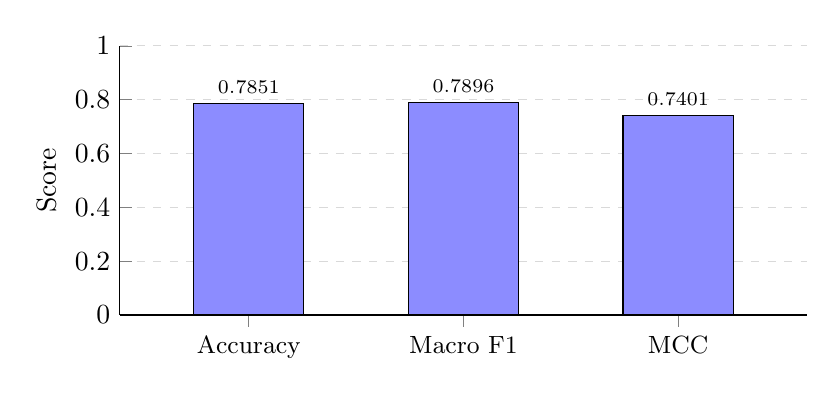
\begin{tikzpicture}
\begin{axis}[
    ybar,
    width=0.85\columnwidth,
    height=5cm,
    bar width=14mm,
    ymin=0, ymax=1,
    ylabel={Score},
    symbolic x coords={Accuracy,Macro F1,MCC},
    xtick=data,
    x tick label style={font=\small},
    nodes near coords={\pgfmathprintnumber[fixed,precision=4]{\pgfplotspointmeta}},
    nodes near coords style={font=\scriptsize},
    enlarge x limits=0.3,
    ymajorgrids, grid style={dashed, gray!30},
    axis lines*=left,
    clip=false
]
\addplot[fill=blue!45] coordinates {
    (Accuracy,0.7851)
    (Macro F1,0.7896)
    (MCC,0.7401)
};
\end{axis}
\end{tikzpicture}
\caption{Aggregate performance of the supplementary XGBoost classifier on the 470-tenant out-of-distribution holdout: overall accuracy, macro-averaged F1, and Matthews correlation coefficient (MCC).}
\label{fig:accuracy}
\end{figure}

By global mean absolute SHAP value, the three most influential features are the number of distinct \textsc{Critical} rules fired, the total violation count, and the maximum individual rule score, consistent with the rule engine's own severity-floor design: findings that would clamp the deterministic score are also the features the classifier relies on most.

\subsection{System Validation}
\label{sec:systemval}
The deterministic rule engine's reproducibility and cross-tenant isolation are tested directly, independent of its scoring or classification behavior.

\subsubsection{Determinism and Reproducibility}
\label{sec:determinism}
\textbf{Method:} evaluate one tenant end-to-end 100 consecutive times with no change to its input data, comparing the resulting risk score, tier, and violated-rule list across all runs.

\textbf{Result:} all 100 runs produced an identical risk score (65.0), tier (\textsc{High}), and violated-rule list -- zero observed non-determinism in the core evaluation logic.

\subsubsection{Tenant Isolation}
\label{sec:isolation}
\textbf{Method:} evaluate three named tenants (Tenant A, Tenant B, Tenant E), modify only Tenant E's underlying records, and re-evaluate all three.

\textbf{Result:} Tenant E's score changed as expected, from 45.0 to 1.4. Tenant A and Tenant B were unaffected, retaining an identical risk score (65.0) and an identical violated-rule list across both runs -- directly confirming isolation for the tenants tested.

\section{Limitations}
\label{sec:limitations}
\textbf{Structured evidence, not unstructured documents.} \system{} operates on structured relational and transactional tenant records (Section~\ref{sec:architecture}); it does not perform natural-language extraction from unstructured contracts or PDF policy documents, and its findings are only as complete as the structured evidence supplied to it.

\textbf{Synthetic data by necessity.} DPDP and sectoral banking-privacy restrictions prohibit the use of live customer records for development and validation. Every dataset used in this paper -- the named demonstration tenants and the synthetic training and holdout corpora -- is synthetic or drawn from named demonstration tenants, not real account holders; Section~\ref{sec:threats} discusses the resulting limits on external validity.

\textbf{Decision support, not adjudication.} The rule engine is an automated decision-support tool that operationalizes selected interpretations of DPDP obligations (Section~\ref{sec:threats}, Construct Validity). Its output is not a legal determination and does not substitute for review by a qualified compliance or legal professional.

\textbf{Knowledge-base currency.} The 16-rule, 3-policy knowledge base reflects the Act and rules in force at the time of writing. New rules notified by the Data Protection Board will require corresponding knowledge-base updates, tracked through the versioning discussed under Operational Validity (Section~\ref{sec:threats}).

\textbf{Retention and deletion tooling.} As reported in Section~\ref{sec:retention}, mapped tenant data has no automated retention time-to-live and no application-level, audit-logged deletion endpoint; purging a tenant currently requires direct backend or database access.

\section{Threats to Validity}
\label{sec:threats}
\textbf{Construct validity:} Codified rules operationalize selected interpretations of statutory obligations. A correct implementation of a rule is not automatically a legally authoritative interpretation. Future review should involve qualified domain experts and maintain traceability from each rule to the relevant statutory text.

\textbf{Internal validity:} The compliancy-validation, risk-scoring, and system-validation exercises reported in Section~\ref{sec:validation} are each limited to a small number of hand-selected tenants, conditions, and adversarial inputs, so they establish existence rather than exhaustive generality across the full space of tenants and rule combinations.

\textbf{External validity:} The demonstration tenants and the synthetic training and holdout corpora used in this paper do not represent a probability sample of Indian fintech organizations. No conclusion about industry-wide compliance follows from them.

\textbf{Conclusion validity:} Findings that hold on a small, hand-selected set of tenants and conditions are not automatically general. The determinism, isolation, sensitivity, score-spread, and compliancy-validation results reported here are exact and reproducible for the cases tested, and this paper does not extrapolate from them to an unqualified population-level conformance claim.

\textbf{Operational validity:} The Act, associated rules, organizational practices, and the project's knowledge base can evolve. Versioning the statute mapping, rules, schemas, and models is necessary so an old report can be reconstructed under the artifacts in force when it was generated.

\section{Conclusion}
This paper presented \system, a hybrid DPDP compliance-assessment framework built around deterministic evidence evaluation, opportunity-aware risk scoring, and a supplementary explainable classifier. Its validation spans four independent streams, each reporting concrete, directly measured evidence. Compliancy validation confirmed data minimization, pseudonymization, retention and deletion behavior, authentication and authorization, and end-to-end data integrity, using canary-value tracing, adversarial inputs, and direct database verification rather than reliance on the application's own reported behavior. Risk-scoring and evaluation engine validation confirmed the critical and high-count severity floors, monotonicity, and a non-degenerate, genuinely differentiated score across independently constructed tenants. ML layer validation evaluated the supplementary XGBoost classifier on a 470-tenant out-of-distribution holdout, structurally decorrelated from its training corpus, achieving a Macro F1 of 0.7896 and a Matthews correlation coefficient of 0.7401, with every misclassification confined to an adjacent risk tier. System validation confirmed the deterministic rule engine is reproducible across 100 repeated runs of the same tenant and isolates tenants from each other's evidence. Together, these four streams give \system{} an evidence base that spans its machine-learning component, its deterministic decision logic, and the system that operationalizes both.

\section*{Declarations}
\noindent\textbf{Conflict of interest:} The authors declare no conflict of interest.

\noindent\textbf{Data availability:} The code and datasets supporting this study are available from the corresponding author upon reasonable request.

\begin{thebibliography}{00}

\bibitem{dpdp}
Ministry of Law and Justice, Government of India, ``The Digital Personal Data Protection Act, 2023,'' Act No.~22 of 2023, Aug. 11, 2023.

\bibitem{hamdani}
R. El Hamdani, M. Mustapha, D. R. Amariles, A. Troussel, S. Meeus, and K. Krasnashchok, ``A combined rule-based and machine learning approach for automated GDPR compliance checking,'' in \emph{Proc. 18th Int. Conf. Artificial Intelligence and Law}, 2021, pp. 40--49, doi: 10.1145/3462757.3466081. \url{https://doi.org/10.1145/3462757.3466081}

\bibitem{amaral}
O. Amaral, M. I. Azeem, S. Abualhaija, and L. C. Briand, ``NLP-based automated compliance checking of data processing agreements against GDPR,'' \emph{IEEE Trans. Software Eng.}, vol. 49, no. 9, pp. 4282--4303, 2023, doi: 10.1109/TSE.2023.3288901. \url{https://doi.org/10.1109/TSE.2023.3288901}

\bibitem{bonatti}
P. A. Bonatti, S. Kirrane, I. M. Petrova, and L. Sauro, ``Machine understandable policies and GDPR compliance checking,'' arXiv:2001.08930, 2020. \url{https://arxiv.org/abs/2001.08930}

\bibitem{chhetri}
T. R. Chhetri, A. Kurteva, R. J. DeLong, R. Hilscher, K. Korte, and A. Fensel, ``Data protection by design tool for automated GDPR compliance verification based on semantically modeled informed consent,'' \emph{Sensors}, vol. 22, no. 7, Art. no. 2763, 2022.

\bibitem{barr}
E. T. Barr, M. Harman, P. McMinn, M. Shahbaz, and S. Yoo, ``The oracle problem in software testing: A survey,'' \emph{IEEE Trans. Software Eng.}, vol. 41, no. 5, pp. 507--525, May 2015, doi: 10.1109/TSE.2014.2372785. \url{https://doi.org/10.1109/TSE.2014.2372785}

\bibitem{lundberg2017}
S. M. Lundberg and S.-I. Lee, ``A unified approach to interpreting model predictions,'' in \emph{Advances in Neural Information Processing Systems 30}, 2017.

\bibitem{lundberg2020}
S. M. Lundberg \emph{et al.}, ``From local explanations to global understanding with explainable AI for trees,'' \emph{Nature Mach. Intell.}, vol. 2, no. 1, pp. 56--67, 2020.

\bibitem{ribeiro}
M. T. Ribeiro, S. Singh, and C. Guestrin, ``Why should I trust you?: Explaining the predictions of any classifier,'' in \emph{Proc. 22nd ACM SIGKDD Int. Conf. Knowledge Discovery and Data Mining}, 2016, pp. 1135--1144.

\bibitem{xgboost}
T. Chen and C. Guestrin, ``XGBoost: A scalable tree boosting system,'' in \emph{Proc. 22nd ACM SIGKDD Int. Conf. Knowledge Discovery and Data Mining}, 2016, pp. 785--794, doi: 10.1145/2939672.2939785. \url{https://doi.org/10.1145/2939672.2939785}

\bibitem{smote}
N. V. Chawla, K. W. Bowyer, L. O. Hall, and W. P. Kegelmeyer, ``SMOTE: Synthetic minority over-sampling technique,'' \emph{J. Artif. Intell. Res.}, vol. 16, pp. 321--357, 2002, doi: 10.1613/jair.953. \url{https://doi.org/10.1613/jair.953}

\bibitem{kuhn2013}
D. R. Kuhn, R. N. Kacker, and Y. Lei, \emph{Introduction to Combinatorial Testing}. Boca Raton, FL, USA: CRC Press, 2013.

\bibitem{hmac}
H. Krawczyk, M. Bellare, and R. Canetti, ``HMAC: Keyed-Hashing for Message Authentication,'' IETF RFC 2104, Feb. 1997. \url{https://www.rfc-editor.org/rfc/rfc2104}

\bibitem{jwt}
M. Jones, J. Bradley, and N. Sakimura, ``JSON Web Token (JWT),'' IETF RFC 7519, May 2015. \url{https://www.rfc-editor.org/rfc/rfc7519}

\end{thebibliography}

\end{document}
